\documentclass[]{article}
\usepackage{lmodern}
\usepackage{amssymb,amsmath}
\usepackage{ifxetex,ifluatex}
\usepackage{fixltx2e} % provides \textsubscript
\ifnum 0\ifxetex 1\fi\ifluatex 1\fi=0 % if pdftex
  \usepackage[T1]{fontenc}
  \usepackage[utf8]{inputenc}
\else % if luatex or xelatex
  \ifxetex
    \usepackage{mathspec}
  \else
    \usepackage{fontspec}
  \fi
  \defaultfontfeatures{Ligatures=TeX,Scale=MatchLowercase}
\fi
% use upquote if available, for straight quotes in verbatim environments
\IfFileExists{upquote.sty}{\usepackage{upquote}}{}
% use microtype if available
\IfFileExists{microtype.sty}{%
\usepackage{microtype}
\UseMicrotypeSet[protrusion]{basicmath} % disable protrusion for tt fonts
}{}
\usepackage[margin=1in]{geometry}
\usepackage{hyperref}
\hypersetup{unicode=true,
            pdftitle={FINAL PROJECT\_120919 YMaze\_SA Cyt1 flfl},
            pdfauthor={Jacqueline Welday},
            pdfborder={0 0 0},
            breaklinks=true}
\urlstyle{same}  % don't use monospace font for urls
\usepackage{color}
\usepackage{fancyvrb}
\newcommand{\VerbBar}{|}
\newcommand{\VERB}{\Verb[commandchars=\\\{\}]}
\DefineVerbatimEnvironment{Highlighting}{Verbatim}{commandchars=\\\{\}}
% Add ',fontsize=\small' for more characters per line
\usepackage{framed}
\definecolor{shadecolor}{RGB}{248,248,248}
\newenvironment{Shaded}{\begin{snugshade}}{\end{snugshade}}
\newcommand{\AlertTok}[1]{\textcolor[rgb]{0.94,0.16,0.16}{#1}}
\newcommand{\AnnotationTok}[1]{\textcolor[rgb]{0.56,0.35,0.01}{\textbf{\textit{#1}}}}
\newcommand{\AttributeTok}[1]{\textcolor[rgb]{0.77,0.63,0.00}{#1}}
\newcommand{\BaseNTok}[1]{\textcolor[rgb]{0.00,0.00,0.81}{#1}}
\newcommand{\BuiltInTok}[1]{#1}
\newcommand{\CharTok}[1]{\textcolor[rgb]{0.31,0.60,0.02}{#1}}
\newcommand{\CommentTok}[1]{\textcolor[rgb]{0.56,0.35,0.01}{\textit{#1}}}
\newcommand{\CommentVarTok}[1]{\textcolor[rgb]{0.56,0.35,0.01}{\textbf{\textit{#1}}}}
\newcommand{\ConstantTok}[1]{\textcolor[rgb]{0.00,0.00,0.00}{#1}}
\newcommand{\ControlFlowTok}[1]{\textcolor[rgb]{0.13,0.29,0.53}{\textbf{#1}}}
\newcommand{\DataTypeTok}[1]{\textcolor[rgb]{0.13,0.29,0.53}{#1}}
\newcommand{\DecValTok}[1]{\textcolor[rgb]{0.00,0.00,0.81}{#1}}
\newcommand{\DocumentationTok}[1]{\textcolor[rgb]{0.56,0.35,0.01}{\textbf{\textit{#1}}}}
\newcommand{\ErrorTok}[1]{\textcolor[rgb]{0.64,0.00,0.00}{\textbf{#1}}}
\newcommand{\ExtensionTok}[1]{#1}
\newcommand{\FloatTok}[1]{\textcolor[rgb]{0.00,0.00,0.81}{#1}}
\newcommand{\FunctionTok}[1]{\textcolor[rgb]{0.00,0.00,0.00}{#1}}
\newcommand{\ImportTok}[1]{#1}
\newcommand{\InformationTok}[1]{\textcolor[rgb]{0.56,0.35,0.01}{\textbf{\textit{#1}}}}
\newcommand{\KeywordTok}[1]{\textcolor[rgb]{0.13,0.29,0.53}{\textbf{#1}}}
\newcommand{\NormalTok}[1]{#1}
\newcommand{\OperatorTok}[1]{\textcolor[rgb]{0.81,0.36,0.00}{\textbf{#1}}}
\newcommand{\OtherTok}[1]{\textcolor[rgb]{0.56,0.35,0.01}{#1}}
\newcommand{\PreprocessorTok}[1]{\textcolor[rgb]{0.56,0.35,0.01}{\textit{#1}}}
\newcommand{\RegionMarkerTok}[1]{#1}
\newcommand{\SpecialCharTok}[1]{\textcolor[rgb]{0.00,0.00,0.00}{#1}}
\newcommand{\SpecialStringTok}[1]{\textcolor[rgb]{0.31,0.60,0.02}{#1}}
\newcommand{\StringTok}[1]{\textcolor[rgb]{0.31,0.60,0.02}{#1}}
\newcommand{\VariableTok}[1]{\textcolor[rgb]{0.00,0.00,0.00}{#1}}
\newcommand{\VerbatimStringTok}[1]{\textcolor[rgb]{0.31,0.60,0.02}{#1}}
\newcommand{\WarningTok}[1]{\textcolor[rgb]{0.56,0.35,0.01}{\textbf{\textit{#1}}}}
\usepackage{graphicx}
% grffile has become a legacy package: https://ctan.org/pkg/grffile
\IfFileExists{grffile.sty}{%
\usepackage{grffile}
}{}
\makeatletter
\def\maxwidth{\ifdim\Gin@nat@width>\linewidth\linewidth\else\Gin@nat@width\fi}
\def\maxheight{\ifdim\Gin@nat@height>\textheight\textheight\else\Gin@nat@height\fi}
\makeatother
% Scale images if necessary, so that they will not overflow the page
% margins by default, and it is still possible to overwrite the defaults
% using explicit options in \includegraphics[width, height, ...]{}
\setkeys{Gin}{width=\maxwidth,height=\maxheight,keepaspectratio}
\IfFileExists{parskip.sty}{%
\usepackage{parskip}
}{% else
\setlength{\parindent}{0pt}
\setlength{\parskip}{6pt plus 2pt minus 1pt}
}
\setlength{\emergencystretch}{3em}  % prevent overfull lines
\providecommand{\tightlist}{%
  \setlength{\itemsep}{0pt}\setlength{\parskip}{0pt}}
\setcounter{secnumdepth}{0}
% Redefines (sub)paragraphs to behave more like sections
\ifx\paragraph\undefined\else
\let\oldparagraph\paragraph
\renewcommand{\paragraph}[1]{\oldparagraph{#1}\mbox{}}
\fi
\ifx\subparagraph\undefined\else
\let\oldsubparagraph\subparagraph
\renewcommand{\subparagraph}[1]{\oldsubparagraph{#1}\mbox{}}
\fi

%%% Use protect on footnotes to avoid problems with footnotes in titles
\let\rmarkdownfootnote\footnote%
\def\footnote{\protect\rmarkdownfootnote}

%%% Change title format to be more compact
\usepackage{titling}

% Create subtitle command for use in maketitle
\providecommand{\subtitle}[1]{
  \posttitle{
    \begin{center}\large#1\end{center}
    }
}

\setlength{\droptitle}{-2em}

  \title{FINAL PROJECT\_120919 YMaze\_SA Cyt1 flfl}
    \pretitle{\vspace{\droptitle}\centering\huge}
  \posttitle{\par}
    \author{Jacqueline Welday}
    \preauthor{\centering\large\emph}
  \postauthor{\par}
    \date{}
    \predate{}\postdate{}
  

\begin{document}
\maketitle

\hypertarget{introduction}{%
\subsection{Introduction}\label{introduction}}

\hypertarget{import-data}{%
\subsection{Import Data}\label{import-data}}

\begin{Shaded}
\begin{Highlighting}[]
\CommentTok{##install.packages('tidyverse')}
\KeywordTok{library}\NormalTok{ (tidyverse)}
\CommentTok{##install.packages('ggplot2')}
\KeywordTok{library}\NormalTok{ (ggplot2)}
\CommentTok{#install.packages('dplyr')}
\KeywordTok{library}\NormalTok{(dplyr)}
\CommentTok{##install.packages('readxl')}
\KeywordTok{library}\NormalTok{ (rio)}

\CommentTok{## load csv files - the input file name has to be updates each time and the file needs to be in the same project folder than the code}
\NormalTok{data <-}\StringTok{ }\KeywordTok{read_csv}\NormalTok{(}\StringTok{"102819 YMaze_SA Cyt1 flfl Data_Seq.csv"}\NormalTok{,)}
\KeywordTok{head}\NormalTok{(data)}
\end{Highlighting}
\end{Shaded}

\begin{verbatim}
## # A tibble: 6 x 129
##    Test Animal Treatment Time  Date  Distance `Visited zones` X8    X9    X10  
##   <dbl>  <dbl> <chr>     <tim> <chr>    <dbl> <chr>           <chr> <chr> <chr>
## 1     1   4667 Cre       12:14 10/2~    11.4  Arm 1           Cent~ Arm 1 Cent~
## 2     2   4668 ctrl      12:21 10/2~    14.4  Arm 1           Cent~ Arm 3 Cent~
## 3     3   4669 ctrl      12:28 10/2~    14.3  Arm 1           Cent~ Arm 3 Cent~
## 4     4   5054 cre       12:36 10/2~    14.4  Arm 1           Cent~ Arm 3 Cent~
## 5     5   5055 ctrl      12:43 10/2~    12.8  Arm 1           Cent~ Arm 2 Cent~
## 6     6   4673 cre       12:50 10/2~     9.71 Arm 1           Cent~ Arm 3 Cent~
## # ... with 119 more variables: X11 <chr>, X12 <chr>, X13 <chr>, X14 <chr>,
## #   X15 <chr>, X16 <chr>, X17 <chr>, X18 <chr>, X19 <chr>, X20 <chr>,
## #   X21 <chr>, X22 <chr>, X23 <chr>, X24 <chr>, X25 <chr>, X26 <chr>,
## #   X27 <chr>, X28 <chr>, X29 <chr>, X30 <chr>, X31 <chr>, X32 <chr>,
## #   X33 <chr>, X34 <chr>, X35 <chr>, X36 <chr>, X37 <chr>, X38 <chr>,
## #   X39 <chr>, X40 <chr>, X41 <chr>, X42 <chr>, X43 <chr>, X44 <chr>,
## #   X45 <chr>, X46 <chr>, X47 <chr>, X48 <chr>, X49 <chr>, X50 <chr>,
## #   X51 <chr>, X52 <chr>, X53 <chr>, X54 <chr>, X55 <chr>, X56 <chr>,
## #   X57 <chr>, X58 <chr>, X59 <chr>, X60 <chr>, X61 <chr>, X62 <chr>,
## #   X63 <chr>, X64 <chr>, X65 <chr>, X66 <chr>, X67 <chr>, X68 <chr>,
## #   X69 <chr>, X70 <chr>, X71 <chr>, X72 <chr>, X73 <chr>, X74 <chr>,
## #   X75 <chr>, X76 <chr>, X77 <chr>, X78 <chr>, X79 <chr>, X80 <chr>,
## #   X81 <chr>, X82 <chr>, X83 <chr>, X84 <chr>, X85 <chr>, X86 <chr>,
## #   X87 <chr>, X88 <chr>, X89 <chr>, X90 <chr>, X91 <chr>, X92 <chr>,
## #   X93 <chr>, X94 <chr>, X95 <chr>, X96 <chr>, X97 <chr>, X98 <chr>,
## #   X99 <chr>, X100 <chr>, X101 <chr>, X102 <chr>, X103 <chr>, X104 <chr>,
## #   X105 <chr>, X106 <chr>, X107 <chr>, X108 <chr>, X109 <chr>, X110 <chr>, ...
\end{verbatim}

\hypertarget{tidying}{%
\subsection{Tidying}\label{tidying}}

\begin{Shaded}
\begin{Highlighting}[]
\NormalTok{n<-}\KeywordTok{nrow}\NormalTok{(data)}

\ControlFlowTok{for}\NormalTok{ (i }\ControlFlowTok{in} \DecValTok{1}\OperatorTok{:}\NormalTok{n)\{}
\NormalTok{  animali<-}\StringTok{ }\NormalTok{data[i,]}
\NormalTok{  animali<-}\StringTok{ }\NormalTok{animali }\OperatorTok\StringTok{ }\KeywordTok{select}\NormalTok{ (}\StringTok{'Visited zones'}\NormalTok{, }\KeywordTok{contains}\NormalTok{(}\StringTok{"X"}\NormalTok{))  }\OperatorTok\StringTok{ }\KeywordTok{gather}\NormalTok{(variable, sequence) }\OperatorTok\StringTok{ }\KeywordTok{select}\NormalTok{(sequence) }\OperatorTok\StringTok{ }\KeywordTok{filter}\NormalTok{(sequence }\OperatorTok{!=}\NormalTok{(}\StringTok{'Center'}\NormalTok{))}
\NormalTok{  animali<-animali }\OperatorTok\StringTok{ }\KeywordTok{mutate}\NormalTok{ (}\DataTypeTok{onebefore=} \KeywordTok{lag}\NormalTok{(sequence)) }\OperatorTok\StringTok{ }\KeywordTok{mutate}\NormalTok{ (}\DataTypeTok{twobefore=}\KeywordTok{lag}\NormalTok{(onebefore)) }\OperatorTok\StringTok{ }\KeywordTok{mutate}\NormalTok{(}\DataTypeTok{threebefore=}\KeywordTok{lag}\NormalTok{(twobefore)) }\OperatorTok\StringTok{ }
\StringTok{    }\KeywordTok{mutate}\NormalTok{ (}\DataTypeTok{alternation1=} \KeywordTok{ifelse}\NormalTok{(sequence}\OperatorTok{==}\StringTok{'Arm 1'}\OperatorTok{&}\StringTok{ }\NormalTok{onebefore}\OperatorTok{==}\StringTok{'Arm 2'} \OperatorTok{&}\StringTok{ }\NormalTok{twobefore}\OperatorTok{==}\StringTok{'Arm 3'}\NormalTok{,}\DecValTok{1}\NormalTok{,}\DecValTok{0}\NormalTok{)) }\OperatorTok\StringTok{ }
\StringTok{    }\KeywordTok{mutate}\NormalTok{ (}\DataTypeTok{alternation2=} \KeywordTok{ifelse}\NormalTok{(sequence}\OperatorTok{==}\StringTok{'Arm 1'}\OperatorTok{&}\StringTok{ }\NormalTok{onebefore}\OperatorTok{==}\StringTok{'Arm 3'} \OperatorTok{&}\StringTok{ }\NormalTok{twobefore}\OperatorTok{==}\StringTok{'Arm 2'}\NormalTok{,}\DecValTok{1}\NormalTok{,}\DecValTok{0}\NormalTok{)) }\OperatorTok\StringTok{ }
\StringTok{    }\KeywordTok{mutate}\NormalTok{ (}\DataTypeTok{alternation3=} \KeywordTok{ifelse}\NormalTok{(sequence}\OperatorTok{==}\StringTok{'Arm 2'}\OperatorTok{&}\StringTok{ }\NormalTok{onebefore}\OperatorTok{==}\StringTok{'Arm 3'} \OperatorTok{&}\StringTok{ }\NormalTok{twobefore}\OperatorTok{==}\StringTok{'Arm 1'}\NormalTok{,}\DecValTok{1}\NormalTok{,}\DecValTok{0}\NormalTok{)) }\OperatorTok\StringTok{ }
\StringTok{    }\KeywordTok{mutate}\NormalTok{ (}\DataTypeTok{alternation4=} \KeywordTok{ifelse}\NormalTok{(sequence}\OperatorTok{==}\StringTok{'Arm 2'}\OperatorTok{&}\StringTok{ }\NormalTok{onebefore}\OperatorTok{==}\StringTok{'Arm 1'} \OperatorTok{&}\StringTok{ }\NormalTok{twobefore}\OperatorTok{==}\StringTok{'Arm 3'}\NormalTok{,}\DecValTok{1}\NormalTok{,}\DecValTok{0}\NormalTok{)) }\OperatorTok\StringTok{ }
\StringTok{    }\KeywordTok{mutate}\NormalTok{ (}\DataTypeTok{alternation5=} \KeywordTok{ifelse}\NormalTok{(sequence}\OperatorTok{==}\StringTok{'Arm 3'}\OperatorTok{&}\StringTok{ }\NormalTok{onebefore}\OperatorTok{==}\StringTok{'Arm 1'} \OperatorTok{&}\StringTok{ }\NormalTok{twobefore}\OperatorTok{==}\StringTok{'Arm 2'}\NormalTok{,}\DecValTok{1}\NormalTok{,}\DecValTok{0}\NormalTok{)) }\OperatorTok\StringTok{ }
\StringTok{    }\KeywordTok{mutate}\NormalTok{ (}\DataTypeTok{alternation6=} \KeywordTok{ifelse}\NormalTok{(sequence}\OperatorTok{==}\StringTok{'Arm 3'}\OperatorTok{&}\StringTok{ }\NormalTok{onebefore}\OperatorTok{==}\StringTok{'Arm 2'} \OperatorTok{&}\StringTok{ }\NormalTok{twobefore}\OperatorTok{==}\StringTok{'Arm 1'}\NormalTok{,}\DecValTok{1}\NormalTok{,}\DecValTok{0}\NormalTok{)) }\OperatorTok\StringTok{ }
\StringTok{    }\KeywordTok{mutate}\NormalTok{ (}\DataTypeTok{alternation7=} \KeywordTok{ifelse}\NormalTok{(sequence}\OperatorTok{==}\StringTok{'Arm 1'}\OperatorTok{&}\StringTok{ }\NormalTok{onebefore}\OperatorTok{==}\StringTok{'Arm 2'} \OperatorTok{&}\StringTok{ }\NormalTok{twobefore}\OperatorTok{==}\StringTok{'Arm 2'} \OperatorTok{&}\StringTok{ }\NormalTok{threebefore}\OperatorTok{==}\StringTok{'Arm 3'}\NormalTok{,}\DecValTok{1}\NormalTok{,}\DecValTok{0}\NormalTok{)) }\OperatorTok\StringTok{ }
\StringTok{    }\KeywordTok{mutate}\NormalTok{ (}\DataTypeTok{alternation8=} \KeywordTok{ifelse}\NormalTok{(sequence}\OperatorTok{==}\StringTok{'Arm 1'}\OperatorTok{&}\StringTok{ }\NormalTok{onebefore}\OperatorTok{==}\StringTok{'Arm 3'} \OperatorTok{&}\StringTok{ }\NormalTok{twobefore}\OperatorTok{==}\StringTok{'Arm 3'} \OperatorTok{&}\StringTok{ }\NormalTok{threebefore}\OperatorTok{==}\StringTok{'Arm 2'}\NormalTok{,}\DecValTok{1}\NormalTok{,}\DecValTok{0}\NormalTok{)) }\OperatorTok\StringTok{ }
\StringTok{    }\KeywordTok{mutate}\NormalTok{ (}\DataTypeTok{alternation9=} \KeywordTok{ifelse}\NormalTok{(sequence}\OperatorTok{==}\StringTok{'Arm 2'}\OperatorTok{&}\StringTok{ }\NormalTok{onebefore}\OperatorTok{==}\StringTok{'Arm 1'} \OperatorTok{&}\StringTok{ }\NormalTok{twobefore}\OperatorTok{==}\StringTok{'Arm 1'} \OperatorTok{&}\StringTok{ }\NormalTok{threebefore}\OperatorTok{==}\StringTok{'Arm 3'}\NormalTok{,}\DecValTok{1}\NormalTok{,}\DecValTok{0}\NormalTok{)) }\OperatorTok\StringTok{ }
\StringTok{    }\KeywordTok{mutate}\NormalTok{ (}\DataTypeTok{alternation10=} \KeywordTok{ifelse}\NormalTok{(sequence}\OperatorTok{==}\StringTok{'Arm 2'}\OperatorTok{&}\StringTok{ }\NormalTok{onebefore}\OperatorTok{==}\StringTok{'Arm 3'} \OperatorTok{&}\StringTok{ }\NormalTok{twobefore}\OperatorTok{==}\StringTok{'Arm 3'} \OperatorTok{&}\StringTok{ }\NormalTok{threebefore}\OperatorTok{==}\StringTok{'Arm 1'}\NormalTok{,}\DecValTok{1}\NormalTok{,}\DecValTok{0}\NormalTok{)) }\OperatorTok\StringTok{ }
\StringTok{    }\KeywordTok{mutate}\NormalTok{ (}\DataTypeTok{alternation11=} \KeywordTok{ifelse}\NormalTok{(sequence}\OperatorTok{==}\StringTok{'Arm 3'}\OperatorTok{&}\StringTok{ }\NormalTok{onebefore}\OperatorTok{==}\StringTok{'Arm 2'} \OperatorTok{&}\StringTok{ }\NormalTok{twobefore}\OperatorTok{==}\StringTok{'Arm 2'} \OperatorTok{&}\StringTok{ }\NormalTok{threebefore}\OperatorTok{==}\StringTok{'Arm 1'}\NormalTok{,}\DecValTok{1}\NormalTok{,}\DecValTok{0}\NormalTok{)) }\OperatorTok\StringTok{ }
\StringTok{    }\KeywordTok{mutate}\NormalTok{ (}\DataTypeTok{alternation12=} \KeywordTok{ifelse}\NormalTok{(sequence}\OperatorTok{==}\StringTok{'Arm 3'}\OperatorTok{&}\StringTok{ }\NormalTok{onebefore}\OperatorTok{==}\StringTok{'Arm 1'} \OperatorTok{&}\StringTok{ }\NormalTok{twobefore}\OperatorTok{==}\StringTok{'Arm 1'} \OperatorTok{&}\StringTok{ }\NormalTok{threebefore}\OperatorTok{==}\StringTok{'Arm 2'}\NormalTok{,}\DecValTok{1}\NormalTok{,}\DecValTok{0}\NormalTok{)) }\OperatorTok\StringTok{   }
\StringTok{    }
\StringTok{    }\KeywordTok{mutate}\NormalTok{(}\DataTypeTok{A1=}\KeywordTok{as.numeric}\NormalTok{(alternation1)) }\OperatorTok\StringTok{ }
\StringTok{    }\KeywordTok{mutate}\NormalTok{(}\DataTypeTok{A2=}\KeywordTok{as.numeric}\NormalTok{(alternation2)) }\OperatorTok\StringTok{ }
\StringTok{    }\KeywordTok{mutate}\NormalTok{(}\DataTypeTok{A3=}\KeywordTok{as.numeric}\NormalTok{(alternation3)) }\OperatorTok\StringTok{ }
\StringTok{    }\KeywordTok{mutate}\NormalTok{(}\DataTypeTok{A4=}\KeywordTok{as.numeric}\NormalTok{(alternation4)) }\OperatorTok\StringTok{ }
\StringTok{    }\KeywordTok{mutate}\NormalTok{(}\DataTypeTok{A5=}\KeywordTok{as.numeric}\NormalTok{(alternation5)) }\OperatorTok\StringTok{ }
\StringTok{    }\KeywordTok{mutate}\NormalTok{(}\DataTypeTok{A6=}\KeywordTok{as.numeric}\NormalTok{(alternation6)) }\OperatorTok\StringTok{ }
\StringTok{    }\KeywordTok{mutate}\NormalTok{(}\DataTypeTok{A7=}\KeywordTok{as.numeric}\NormalTok{(alternation7)) }\OperatorTok\StringTok{ }
\StringTok{    }\KeywordTok{mutate}\NormalTok{(}\DataTypeTok{A8=}\KeywordTok{as.numeric}\NormalTok{(alternation8)) }\OperatorTok\StringTok{ }
\StringTok{    }\KeywordTok{mutate}\NormalTok{(}\DataTypeTok{A9=}\KeywordTok{as.numeric}\NormalTok{(alternation9)) }\OperatorTok\StringTok{ }
\StringTok{    }\KeywordTok{mutate}\NormalTok{(}\DataTypeTok{A10=}\KeywordTok{as.numeric}\NormalTok{(alternation10)) }\OperatorTok\StringTok{ }
\StringTok{    }\KeywordTok{mutate}\NormalTok{(}\DataTypeTok{A11=}\KeywordTok{as.numeric}\NormalTok{(alternation11)) }\OperatorTok\StringTok{ }
\StringTok{    }\KeywordTok{mutate}\NormalTok{(}\DataTypeTok{A12=}\KeywordTok{as.numeric}\NormalTok{(alternation12)) }\OperatorTok\StringTok{ }
\StringTok{    }
\StringTok{    }\KeywordTok{mutate}\NormalTok{(}\DataTypeTok{alternation=}\NormalTok{A1}\OperatorTok{+}\NormalTok{A2}\OperatorTok{+}\NormalTok{A3}\OperatorTok{+}\NormalTok{A4}\OperatorTok{+}\NormalTok{A5}\OperatorTok{+}\NormalTok{A6}\OperatorTok{+}\NormalTok{A7}\OperatorTok{+}\NormalTok{A8}\OperatorTok{+}\NormalTok{A9}\OperatorTok{+}\NormalTok{A10}\OperatorTok{+}\NormalTok{A11}\OperatorTok{+}\NormalTok{A12) }\OperatorTok\StringTok{ }
\StringTok{    }
\StringTok{    }\KeywordTok{select}\NormalTok{(sequence, onebefore, twobefore, threebefore, alternation)}
\NormalTok{   animali<-animali[}\OperatorTok{-}\KeywordTok{c}\NormalTok{(}\DecValTok{1}\NormalTok{,}\DecValTok{2}\NormalTok{),]}

\NormalTok{  a<-}\KeywordTok{sum}\NormalTok{(animali}\OperatorTok{$}\NormalTok{alternation, }\DataTypeTok{na.rm=}\NormalTok{T)}
  \CommentTok{#a}
\NormalTok{  entries<-}\KeywordTok{nrow}\NormalTok{(animali)}
  \CommentTok{#entries}
\NormalTok{  percentage<-a}\OperatorTok{/}\NormalTok{entries }\OperatorTok{*}\DecValTok{100}
  \CommentTok{#as.numeric(percentage)}
\NormalTok{  ci<-}\KeywordTok{c}\NormalTok{(data}\OperatorTok{$}\NormalTok{Animal[i], data}\OperatorTok{$}\NormalTok{Treatment[i], data}\OperatorTok{$}\NormalTok{Distance[i], entries, percentage)}
  \ControlFlowTok{if}\NormalTok{ (i}\OperatorTok{==}\DecValTok{1}\NormalTok{) \{final<-}\KeywordTok{rbind}\NormalTok{(ci)\} }\ControlFlowTok{else}\NormalTok{ \{final<-}\KeywordTok{rbind}\NormalTok{(final,ci)\}}
\NormalTok{\}}

\KeywordTok{colnames}\NormalTok{(final)<-}\KeywordTok{c}\NormalTok{(}\StringTok{'Animal'}\NormalTok{,}\StringTok{'Treatment'}\NormalTok{,}\StringTok{'Distance'}\NormalTok{,}\StringTok{'Entries'}\NormalTok{,}\StringTok{'Alternation'}\NormalTok{)}
\NormalTok{final<-}\KeywordTok{as.data.frame}\NormalTok{(final)}
\NormalTok{final<-final }\OperatorTok\StringTok{ }\KeywordTok{arrange}\NormalTok{(Animal)}
\NormalTok{final}
\end{Highlighting}
\end{Shaded}

\begin{verbatim}
##    Animal Treatment Distance Entries      Alternation
## 1    4667       Cre   11.376      26 57.6923076923077
## 2    4668      ctrl   14.446      44 47.7272727272727
## 3    4669      ctrl   14.271      30               60
## 4    4670      ctrl   15.424      42 54.7619047619048
## 5    4671       cre    14.41      45 42.2222222222222
## 6    4673       cre    9.707      26 46.1538461538462
## 7    4674      ctrl   16.393      44 45.4545454545455
## 8    4675       cre    13.43      39 46.1538461538462
## 9    4676      ctrl   12.558      30 36.6666666666667
## 10   4677       cre   18.316      47 53.1914893617021
## 11   4678      ctrl   18.774      42 45.2380952380952
## 12   4679      ctrl   16.943      43 46.5116279069767
## 13   4696       cre    8.588      23 30.4347826086957
## 14   4700       cre   17.731      47 53.1914893617021
## 15   4701       cre   25.909      60               55
## 16   4702      ctrl   19.978      52               50
## 17   5054       cre   14.377      32           59.375
## 18   5055      ctrl   12.845      41 43.9024390243902
\end{verbatim}

\begin{Shaded}
\begin{Highlighting}[]
\KeywordTok{write.csv}\NormalTok{(final, }\DataTypeTok{file=}\StringTok{"BIOF339 FINAL PROJECT_Ymaze Cyt1 flfl_tidy.csv"}\NormalTok{)}
\end{Highlighting}
\end{Shaded}

\hypertarget{statistical-analysis}{%
\subsection{Statistical Analysis}\label{statistical-analysis}}

\begin{Shaded}
\begin{Highlighting}[]
\NormalTok{final2 <-}\StringTok{ }\NormalTok{final }\OperatorTok\StringTok{ }\KeywordTok{mutate}\NormalTok{(}\DataTypeTok{Treatment=}\KeywordTok{toupper}\NormalTok{(Treatment)) }\OperatorTok\StringTok{ }\KeywordTok{mutate}\NormalTok{(}\DataTypeTok{Treatment=}\KeywordTok{as.factor}\NormalTok{(Treatment)) }\OperatorTok\StringTok{ }\KeywordTok{mutate}\NormalTok{(}\DataTypeTok{Alternation=}\KeywordTok{as.numeric}\NormalTok{(}\KeywordTok{as.character}\NormalTok{(Alternation))) }\OperatorTok\StringTok{ }\KeywordTok{mutate}\NormalTok{(}\DataTypeTok{Distance=}\KeywordTok{as.numeric}\NormalTok{(}\KeywordTok{as.character}\NormalTok{(Distance))) }\OperatorTok\StringTok{ }\KeywordTok{mutate}\NormalTok{(}\DataTypeTok{Animal=}\KeywordTok{as.character}\NormalTok{(Animal)) }\OperatorTok\StringTok{ }\KeywordTok{mutate}\NormalTok{(}\DataTypeTok{Entries=}\KeywordTok{as.numeric}\NormalTok{(}\KeywordTok{as.character}\NormalTok{(Entries)))}

\KeywordTok{str}\NormalTok{(final2)}
\end{Highlighting}
\end{Shaded}

\begin{verbatim}
## 'data.frame':    18 obs. of  5 variables:
##  $ Animal     : chr  "4667" "4668" "4669" "4670" ...
##  $ Treatment  : Factor w/ 2 levels "CRE","CTRL": 1 2 2 2 1 1 2 1 2 1 ...
##  $ Distance   : num  11.4 14.4 14.3 15.4 14.4 ...
##  $ Entries    : num  26 44 30 42 45 26 44 39 30 47 ...
##  $ Alternation: num  57.7 47.7 60 54.8 42.2 ...
\end{verbatim}

\begin{Shaded}
\begin{Highlighting}[]
\NormalTok{YMAze_ttest <-}\StringTok{ }\KeywordTok{t.test}\NormalTok{(Alternation}\OperatorTok{~}\NormalTok{Treatment, }\DataTypeTok{data=}\NormalTok{final2) }\OperatorTok\StringTok{ }
\StringTok{  }\NormalTok{broom}\OperatorTok{::}\KeywordTok{tidy}\NormalTok{()}
\KeywordTok{print}\NormalTok{(YMAze_ttest)}
\end{Highlighting}
\end{Shaded}

\begin{verbatim}
## # A tibble: 1 x 10
##   estimate estimate1 estimate2 statistic p.value parameter conf.low conf.high
##      <dbl>     <dbl>     <dbl>     <dbl>   <dbl>     <dbl>    <dbl>     <dbl>
## 1     1.46      49.3      47.8     0.389   0.703      14.7    -6.56      9.48
## # ... with 2 more variables: method <chr>, alternative <chr>
\end{verbatim}

\begin{Shaded}
\begin{Highlighting}[]
\NormalTok{Distance_ttest <-}\StringTok{ }\KeywordTok{t.test}\NormalTok{(Distance}\OperatorTok{~}\NormalTok{Treatment, }\DataTypeTok{data=}\NormalTok{final2) }\OperatorTok\StringTok{ }
\StringTok{  }\NormalTok{broom}\OperatorTok{::}\KeywordTok{tidy}\NormalTok{()}
\KeywordTok{print}\NormalTok{(Distance_ttest)}
\end{Highlighting}
\end{Shaded}

\begin{verbatim}
## # A tibble: 1 x 10
##   estimate estimate1 estimate2 statistic p.value parameter conf.low conf.high
##      <dbl>     <dbl>     <dbl>     <dbl>   <dbl>     <dbl>    <dbl>     <dbl>
## 1   -0.865      14.9      15.7    -0.443   0.666      11.5    -5.14      3.41
## # ... with 2 more variables: method <chr>, alternative <chr>
\end{verbatim}

\hypertarget{graphs}{%
\subsection{Graphs}\label{graphs}}

\begin{Shaded}
\begin{Highlighting}[]
\NormalTok{sem <-}\StringTok{ }\ControlFlowTok{function}\NormalTok{(x) }\KeywordTok{sqrt}\NormalTok{(}\KeywordTok{var}\NormalTok{(x, }\DataTypeTok{na.rm=}\NormalTok{T)}\OperatorTok{/}\KeywordTok{sum}\NormalTok{(}\OperatorTok{!}\KeywordTok{is.na}\NormalTok{(x)))}
\NormalTok{plot_data <-}\StringTok{ }\NormalTok{final2 }\OperatorTok\StringTok{ }
\StringTok{        }\KeywordTok{group_by}\NormalTok{(Treatment) }\OperatorTok\StringTok{ }
\StringTok{        }\KeywordTok{summarise}\NormalTok{(}\DataTypeTok{meanAlt =} \KeywordTok{mean}\NormalTok{(Alternation), }\DataTypeTok{semAlt=}\KeywordTok{sem}\NormalTok{(Alternation))}
\NormalTok{plot_data}
\end{Highlighting}
\end{Shaded}

\begin{verbatim}
## # A tibble: 2 x 3
##   Treatment meanAlt semAlt
##   <fct>       <dbl>  <dbl>
## 1 CRE          49.3   3.03
## 2 CTRL         47.8   2.22
\end{verbatim}

\begin{Shaded}
\begin{Highlighting}[]
\NormalTok{ttest_plot <-}\StringTok{  }\KeywordTok{ggplot}\NormalTok{(}\DataTypeTok{data =}\NormalTok{ plot_data,}
 \DataTypeTok{mapping =} \KeywordTok{aes}\NormalTok{(}\DataTypeTok{x =}\NormalTok{ Treatment, }\DataTypeTok{y=}\NormalTok{meanAlt, }\DataTypeTok{fill=}\NormalTok{Treatment)) }\OperatorTok{+}
\StringTok{ }\KeywordTok{geom_col}\NormalTok{()}\OperatorTok{+}
\StringTok{   }\KeywordTok{labs}\NormalTok{(}\DataTypeTok{x=} \StringTok{"Treatment"}\NormalTok{, }\DataTypeTok{y=} \StringTok{"Percent Alternation"}\NormalTok{, }\DataTypeTok{title=} \StringTok{"YMAze Spontaneous Alternation Percentage"}\NormalTok{) }\OperatorTok{+}
\StringTok{  }\KeywordTok{geom_errorbar}\NormalTok{(}\KeywordTok{aes}\NormalTok{(}\DataTypeTok{ymin=}\NormalTok{meanAlt }\OperatorTok{-}\StringTok{ }\NormalTok{semAlt, }\DataTypeTok{ymax=}\NormalTok{ meanAlt}\OperatorTok{+}\NormalTok{semAlt)) }\OperatorTok{+}
\StringTok{  }\KeywordTok{ylim}\NormalTok{(}\DecValTok{0}\NormalTok{,}\DecValTok{70}\NormalTok{)}

\NormalTok{ttest_plot <-}\StringTok{ }\NormalTok{ttest_plot }\OperatorTok{+}\StringTok{ }\KeywordTok{geom_point}\NormalTok{(}\DataTypeTok{data=}\NormalTok{final2, }\DataTypeTok{mapping =} \KeywordTok{aes}\NormalTok{(}\DataTypeTok{x=}\NormalTok{Treatment, }\DataTypeTok{y=}\NormalTok{Alternation, }\DataTypeTok{group=}\NormalTok{Treatment), }\DataTypeTok{show.legend =} \OtherTok{FALSE}\NormalTok{)}
\KeywordTok{print}\NormalTok{(ttest_plot)}
\end{Highlighting}
\end{Shaded}

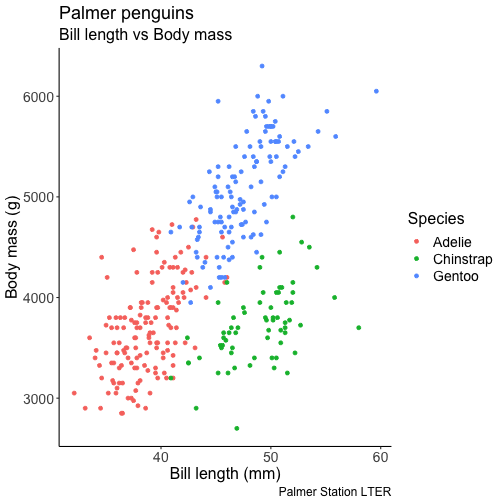
\includegraphics{Welday-Final-Project-BIOF339_files/figure-latex/unnamed-chunk-5-1.pdf}

\begin{Shaded}
\begin{Highlighting}[]
\NormalTok{plot_data_dist <-}\StringTok{ }\NormalTok{final2 }\OperatorTok\StringTok{ }
\StringTok{        }\KeywordTok{group_by}\NormalTok{(Treatment) }\OperatorTok\StringTok{ }
\StringTok{        }\KeywordTok{summarise}\NormalTok{(}\DataTypeTok{meanDist =} \KeywordTok{mean}\NormalTok{(Distance), }\DataTypeTok{semDist=}\KeywordTok{sem}\NormalTok{(Distance))}
\NormalTok{plot_data_dist}
\end{Highlighting}
\end{Shaded}

\begin{verbatim}
## # A tibble: 2 x 3
##   Treatment meanDist semDist
##   <fct>        <dbl>   <dbl>
## 1 CRE           14.9   1.76 
## 2 CTRL          15.7   0.846
\end{verbatim}

\begin{Shaded}
\begin{Highlighting}[]
\NormalTok{distance_plot <-plot_data_dist }\OperatorTok\StringTok{ }
\StringTok{  }\KeywordTok{ggplot}\NormalTok{(}\DataTypeTok{mapping=}\KeywordTok{aes}\NormalTok{(}\DataTypeTok{x=}\NormalTok{Treatment, }\DataTypeTok{y=}\NormalTok{meanDist, }\DataTypeTok{fill=}\NormalTok{Treatment))}\OperatorTok{+}
\StringTok{  }\KeywordTok{geom_col}\NormalTok{()}\OperatorTok{+}
\StringTok{  }\KeywordTok{labs}\NormalTok{(}\DataTypeTok{x=}\StringTok{"Treatment"}\NormalTok{, }\DataTypeTok{y=}\StringTok{"Average Distance (m)"}\NormalTok{, }\DataTypeTok{title=}\StringTok{"Average Distance Travelled by Group"}\NormalTok{)}\OperatorTok{+}
\StringTok{  }\KeywordTok{geom_errorbar}\NormalTok{(}\KeywordTok{aes}\NormalTok{(}\DataTypeTok{ymin=}\NormalTok{meanDist }\OperatorTok{-}\StringTok{ }\NormalTok{semDist, }\DataTypeTok{ymax=}\NormalTok{ meanDist}\OperatorTok{+}\NormalTok{semDist))}

\NormalTok{distance_plot <-}\StringTok{ }\NormalTok{distance_plot }\OperatorTok{+}\StringTok{ }\KeywordTok{geom_point}\NormalTok{(}\DataTypeTok{data=}\NormalTok{final2, }\DataTypeTok{mapping =} \KeywordTok{aes}\NormalTok{(}\DataTypeTok{x=}\NormalTok{Treatment, }\DataTypeTok{y=}\NormalTok{Distance, }\DataTypeTok{group=}\NormalTok{Treatment), }\DataTypeTok{show.legend =} \OtherTok{FALSE}\NormalTok{)}
\KeywordTok{print}\NormalTok{(distance_plot)}
\end{Highlighting}
\end{Shaded}

\includegraphics{Welday-Final-Project-BIOF339_files/figure-latex/unnamed-chunk-5-2.pdf}

\hypertarget{conclusion}{%
\subsection{Conclusion}\label{conclusion}}


\end{document}
